
\section{Experiments}
\label{sec:experiments}

We evaluate the main proposed methods, REPMD and PMAC,
on a number of benchmark tasks against strong baseline methods.
Additional implementation details are provided in \cref{subsec:implementation}. 

\begin{figure*}[t]
\begin{center}
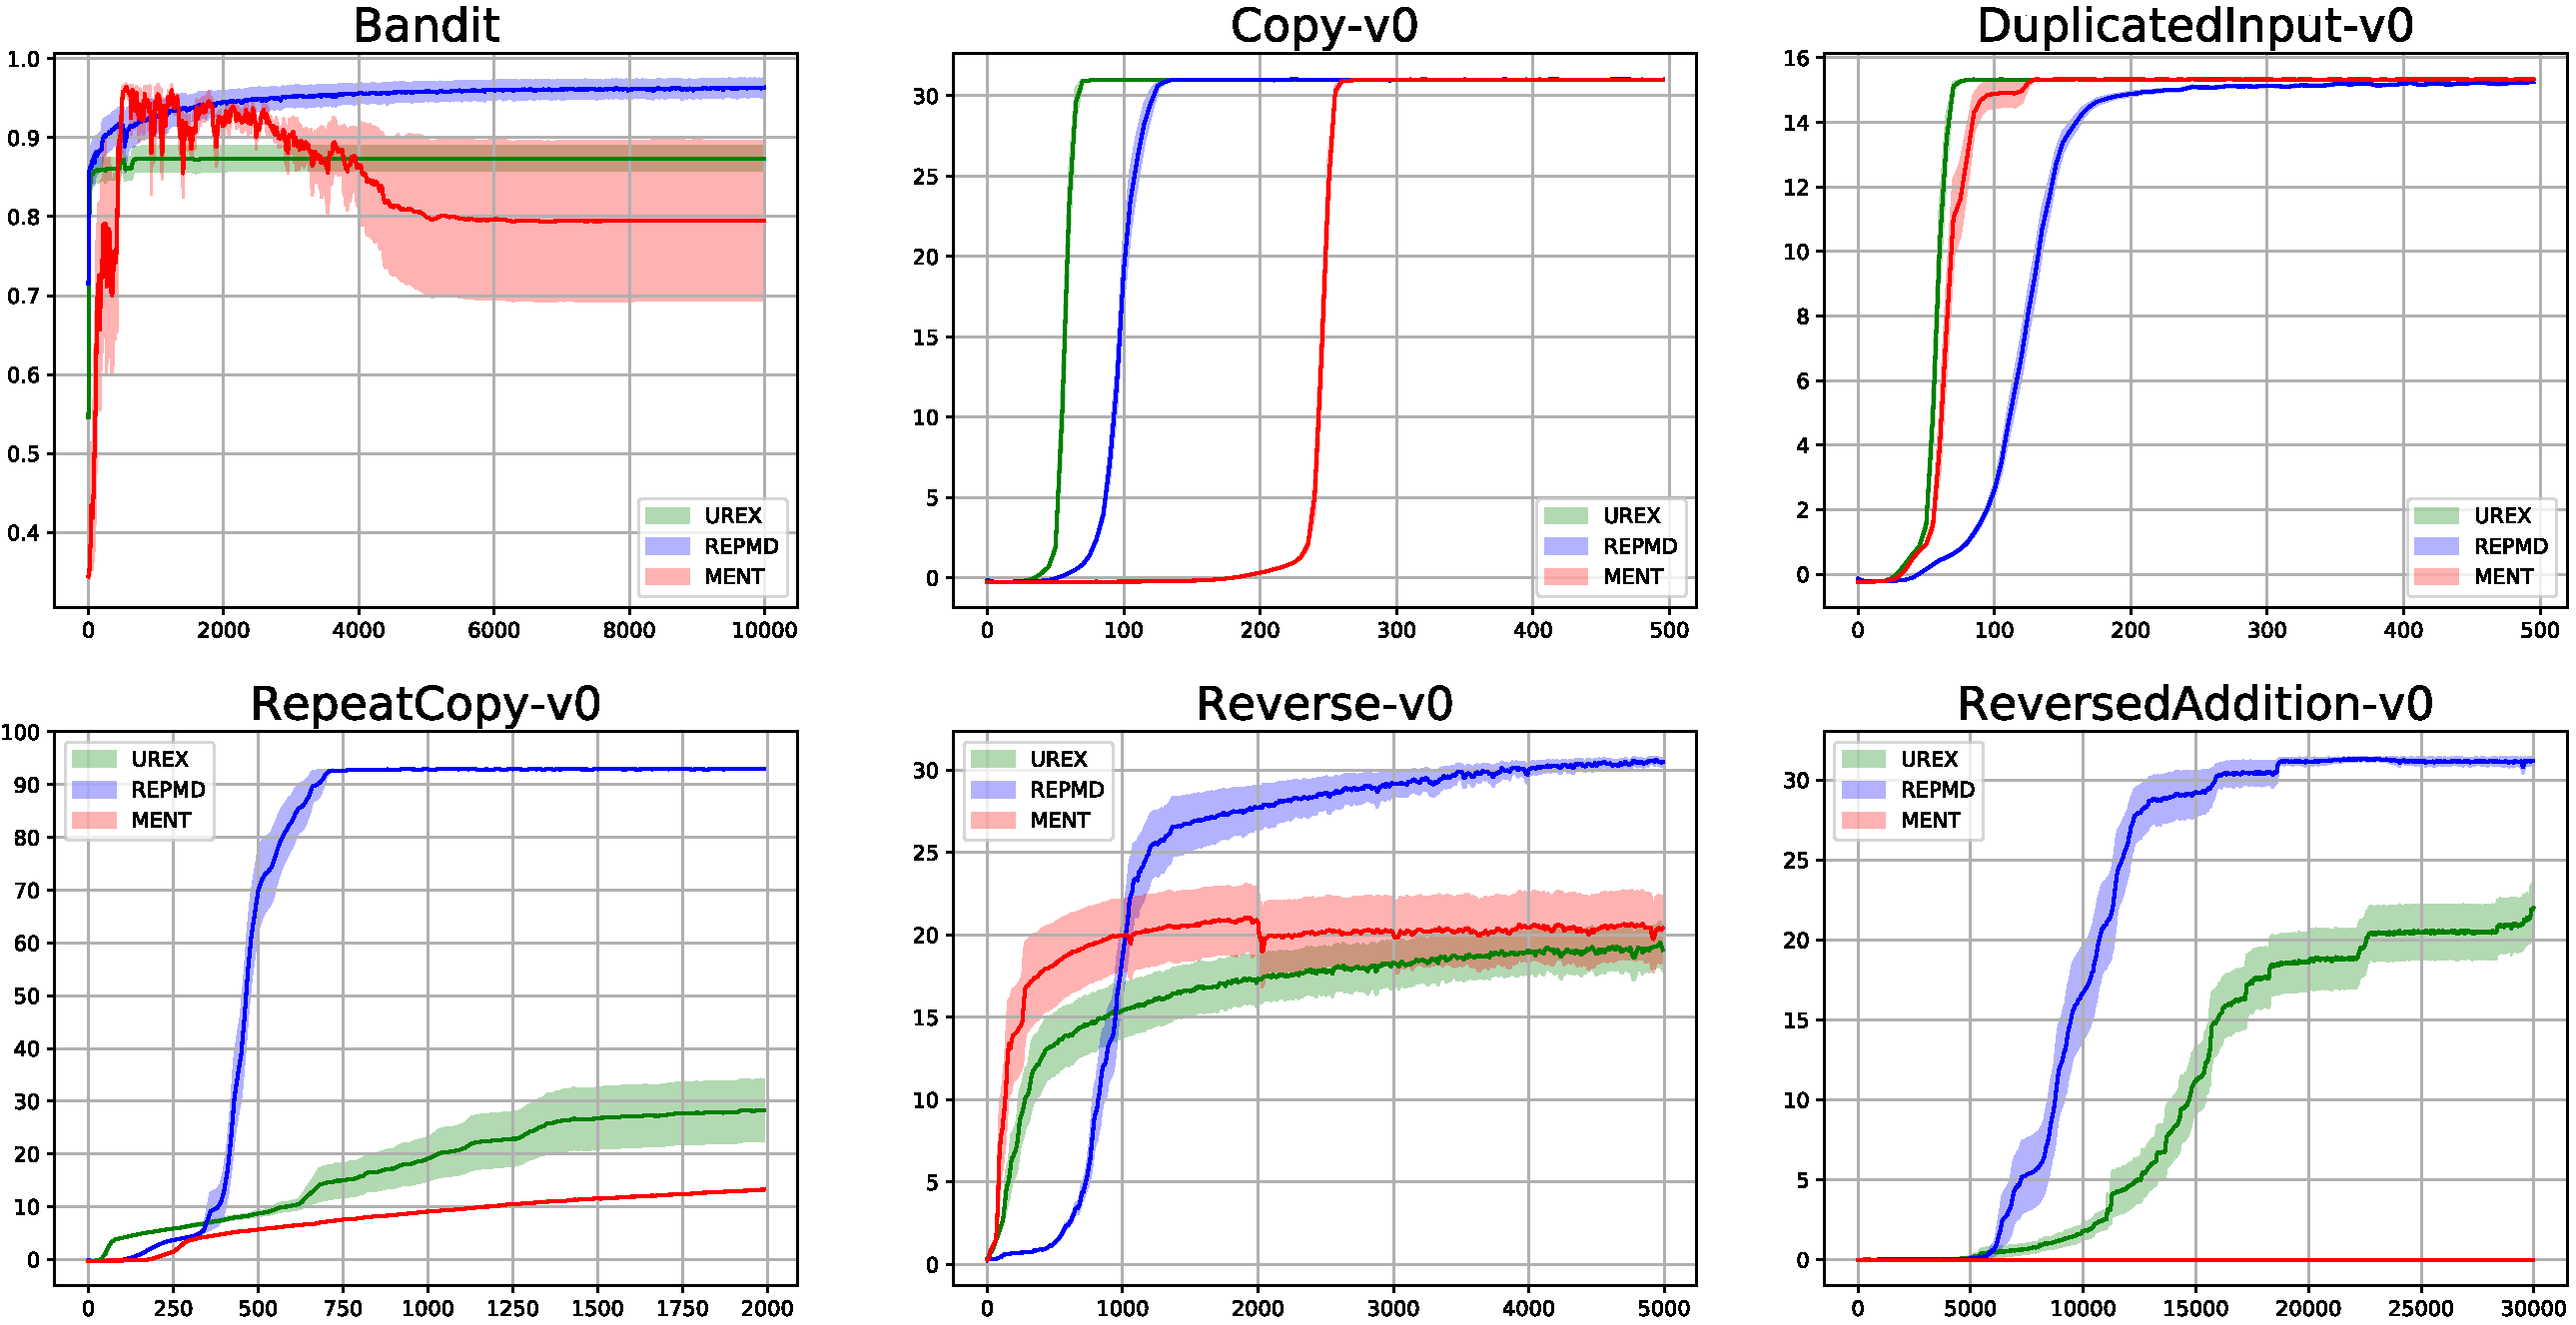
\includegraphics[width=0.75\linewidth]{./bandit_algorithmic_results.pdf}
\end{center}
\caption{
Results of MENT (red), UREX (green), and REPMD (blue) on synthetic bandit
problem and algorithmic tasks.
Plots show average reward with standard error during training.
Synthetic bandit results averaged over 5 runs.
Algorithmic task results averaged over 25 random training runs
(5 runs $\times$ 5 random seeds for neural network initialization).
X-axis is number of sampled trajectories.
} 
\label{fig:results}
\end{figure*}

\subsection{Settings}
\label{subsec:tasks}

We first investigate the performance of REPMD on a synthetic bandit problem
and the algorithmic task suite from the OpenAI gym \citep{brockman2016openai}.
The synthetic multi-armed bandit problem has 10,000 distinct actions,
where
the reward of each action $i$ is initialized by $r_i = s_i^{8}$
such that $s_i$ is randomly sampled from a uniform $[0,1)$ distribution.
Each action $i$ is represented by a randomly sampled feature vector
$\omega_i\in \mathbb{R}^{20}$ from standard normal distribution.
Note that these features are fixed during training.
We further test our method on five algorithmic tasks from the OpenAI gym
library, in rough order of difficulty:
Copy, DuplicatedInput, RepeatCopy, Reverse, and ReversedAddition
\citep{brockman2016openai}.
%
Second, we test the second PMAC approach on continuous-control benchmarks
from OpenAI Gym, utilizing the Mujoco environment
\citep{brockman2016openai,todorov2012mujoco};
including Hopper, Walker2d, HalfCheetah, Ant and Humanoid.
The details of the algorithmic and Mujoco tasks are provided in
\cref{subsec:benchmarks}. 

Note that only cumulative rewards are available in both the
synthetic bandit and algorithmic tasks.
Therefore, value-based RL algorithms can not be applied in this setting.
This restriction compels us to compare REPMD against
REINFORCE with entropy regularization (MENT) \citep{williams1992simple},
and under-appreciated reward exploration (UREX) \citep{nachum2017improving}.
To the best of our knowledge,
these
are the state-of-the-art policy-based algorithms for these algorithmic tasks. 
%
For the continuous control tasks, we compare the second PMAC approach
to deep deterministic policy gradient (DDPG) \citep{lillicrap2015continuous},
an efficient off-policy deep RL methods;
twin delayed deep deterministic policy gradient algorithm (TD3)
\citep{fujimoto2018addressing},
a recent extension to DDPG by applying the double Q-learning trick
to address over-estimation problem when function approximations are adopted;
and Soft-Actor-Critic (SAC) \citep{haarnoja2018soft},
a recent state-of-the-art off-policy algorithm on a number of benchmarks.
All of these algorithms are implemented in \emph{rlkit}.%
%
\footnote{
https://github.com/vitchyr/rlkit
} 
We do not include TRPO and PPO in these experiments,
as their performance is dominated by SAC and TD3,
as shown in \citep{haarnoja2018soft,fujimoto2018addressing}. 


\subsection{Comparative Evaluation}

The results on synthetic bandit problem and algorithmic tasks are reported 
in \cref{fig:results}. 
It is clear that REPMD substantially outperforms the baseline methods
on these tasks.
REPMD appears able to consistently achieve a higher score and
learn substantially faster than UREX.
We also find the performance of UREX is unstable.
On the difficult tasks, including RepeatCopy, Reverse and ReversedAddition,
UREX only finds solutions a few times out of 5 runs for each random seed,
which brings the overall scores down.
This observation explains the gap between the results we find here
and those reported in \citet{nachum2017improving}.%
%
\footnote{
The results reported in \citep{nachum2017improving} are averaged over 
5 runs of random restarting,
while our results are averaged over 25 random training runs
(5 runs $\times$ 5 random seed for neural network initialization). 
}
Note that the performance of REPMD is sill significantly better than
UREX even compared to the results reported in \citet{nachum2017improving}. 

\begin{figure*}[t]
\begin{center}
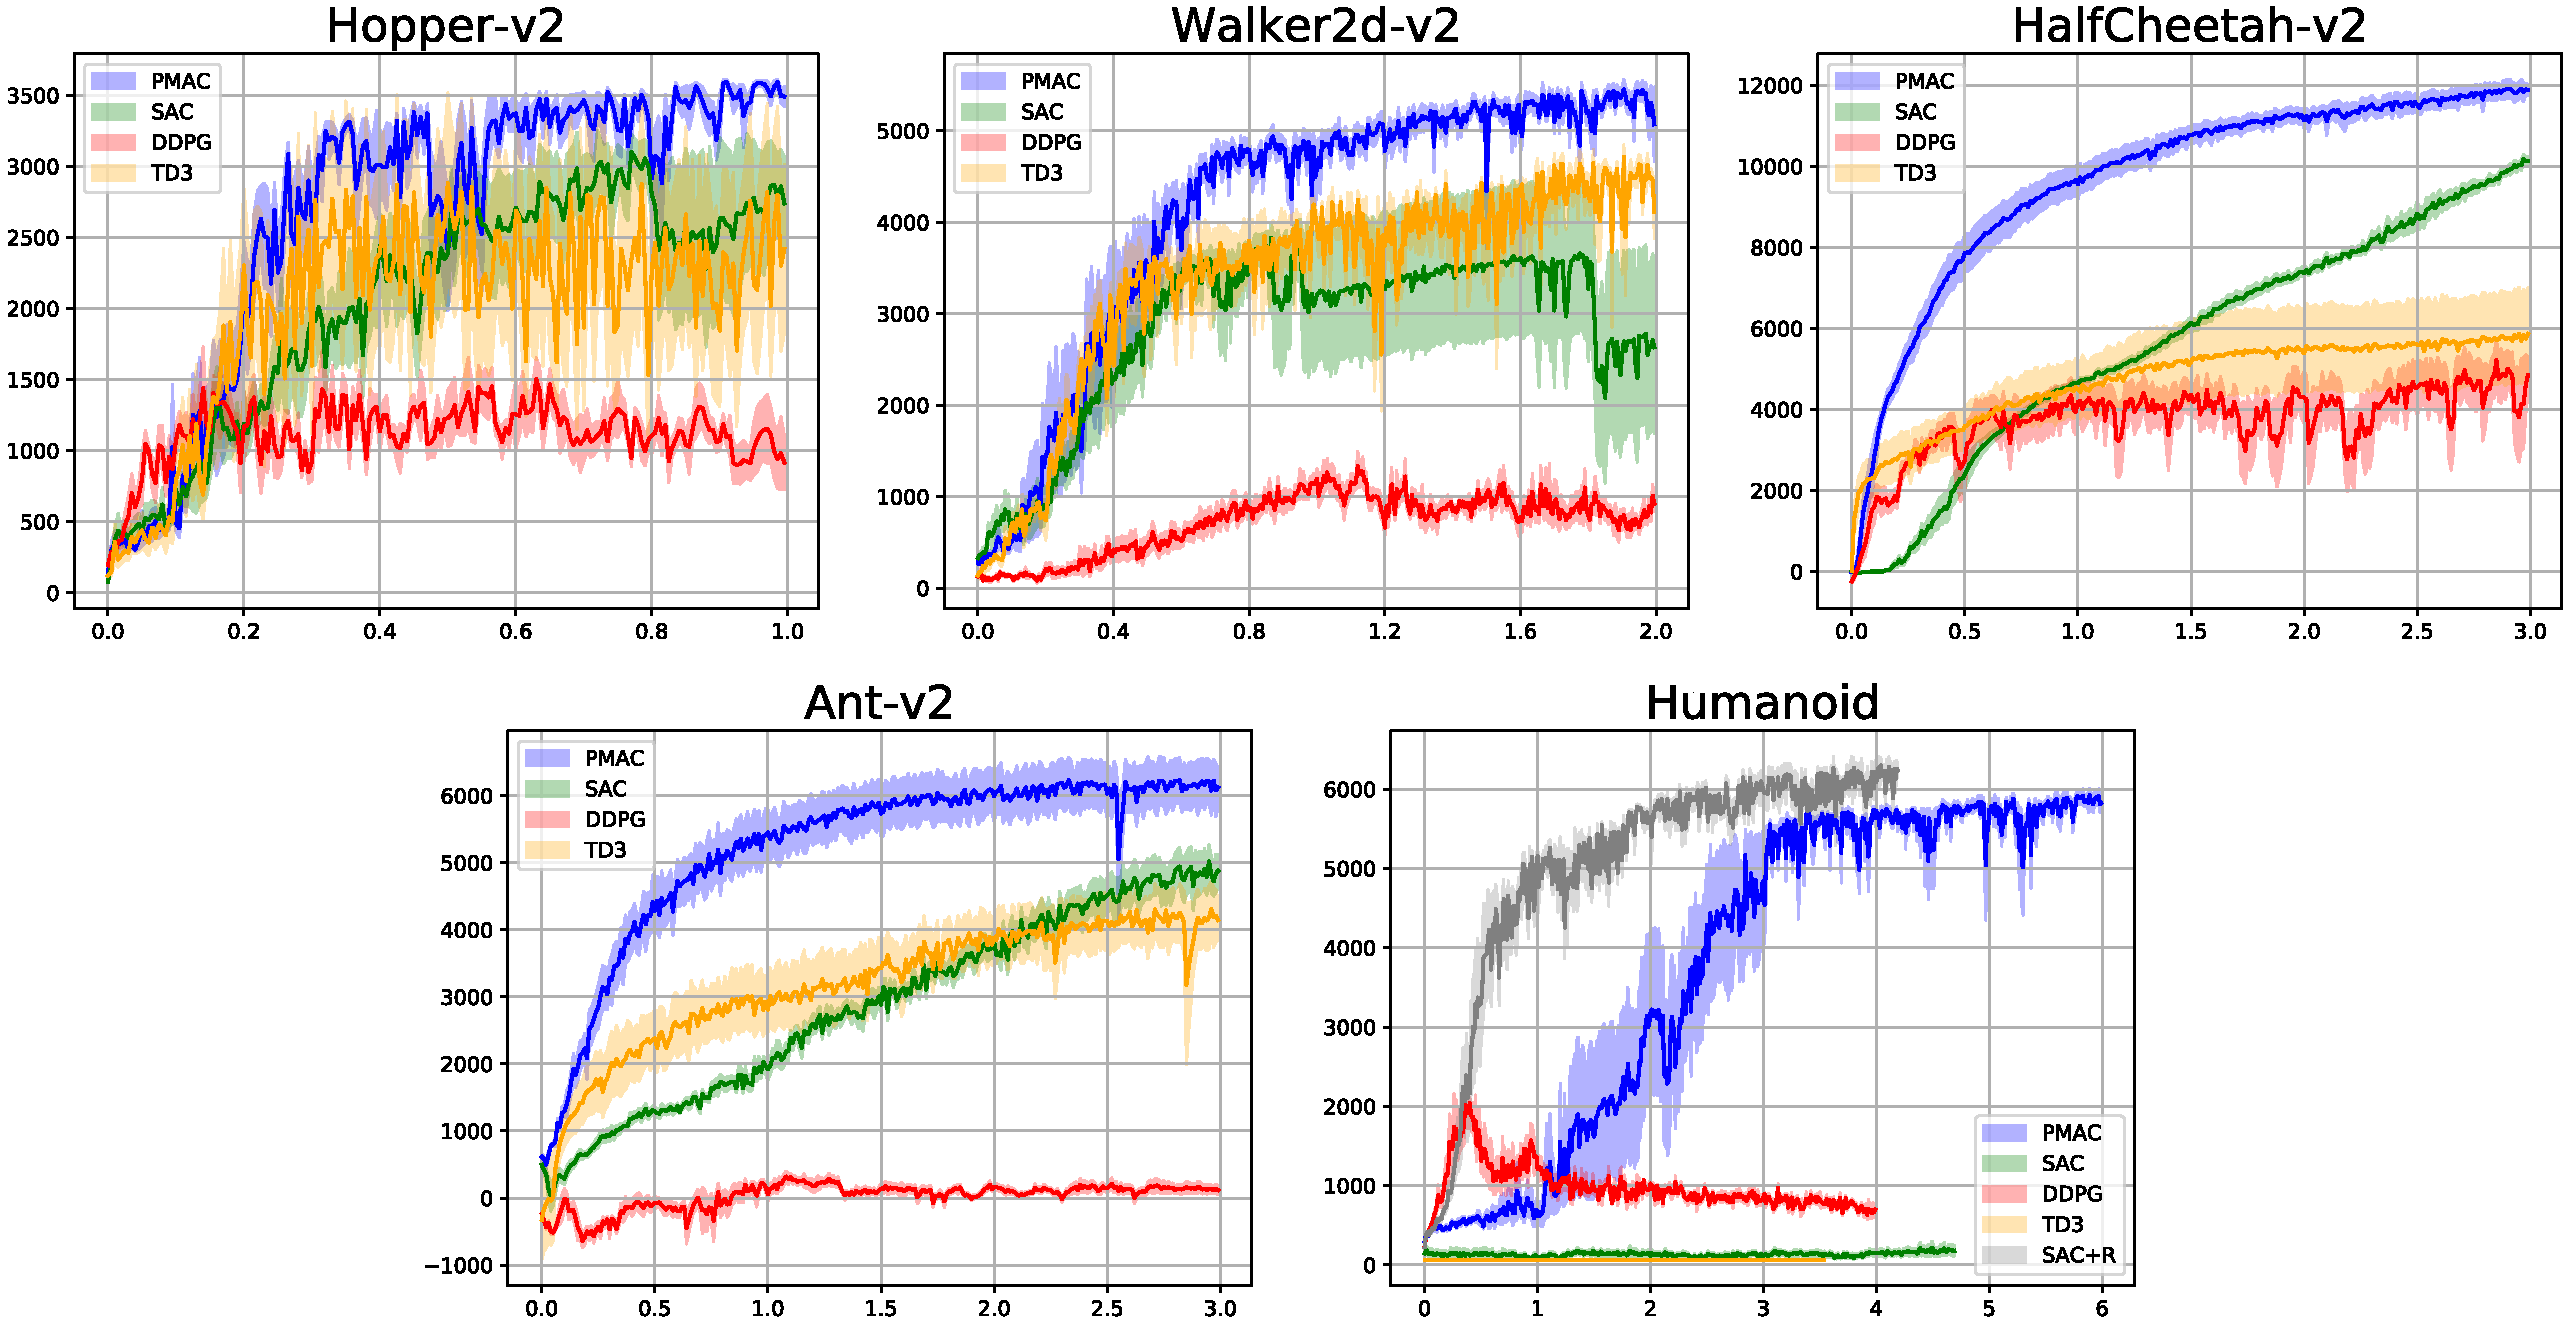
\includegraphics[width=0.8\linewidth]{./mujoco-results.pdf}
\end{center}
\caption{
Learning curves of DDPG (red), TD3 (yellow), SAC (green) and PMAC (blue) on
Mujoco tasks (with SAC+R (gray) added on Humanoid).
Plots show mean reward with standard error during training,
averaged over five different instances with different random seeds.
X-axis is millions of environment steps.
%We observe that PMAC is consistently able to match and, in many cases,
%the performance of the baseline algorithms across all tasks,
%both in terms of final performance and sample efficiency;
%the sole exception being SAC+R on Humanoid.
}
\label{fig:result-mujoco} 
\end{figure*}

\cref{fig:result-mujoco} presents the results on the 
continuous-control benchmarks, reporting the total mean returns
on evaluation rollouts obtained by the algorithms during training.
These
results are averaged over five different instances
with different random seeds.
The solid curves corresponds to the mean and the shaded region to the
standard errors over the five trials.
To ensure a fair comparison with PMAC, we implemented the double-Q
but not the reparameterization trick for SAC 
(see equation (11)-(13) in \citep{haarnoja2018soft}).
This difference explains the discrepancy between the results we see here
and those reported in \citep{haarnoja2018soft}.
We observe that without the reparameterization trick SAC cannot make
any progress in the hardest problem Humanoid.
Therefore, to gain further clarity, 
we also report the result of SAC with the reparameterization trick,
denoted SAC+R,
on Humanoid using the author's GitHub implementation.
The results show that PMAC matches or, in many cases, surpasses all other
baseline algorithms in both final performance and sample efficiency across
tasks, except compared to SAC+R in Humanoid.
In Humanoid, although SAC+R outperforms PMAC,
its final performance is still comparable with SAC+R.
Note that the reparameterization trick that benefits SAC
could also be applied in PMAC;
we have yet to add this modification and
will add this to PMAC in future work.


%\begin{wrapfigure}{R}{0.5\textwidth}
%\label{fig:ablation}
%  \begin{center}
%    \includegraphics[width=0.5\textwidth]{Copy.png}
%  \end{center}
%  \caption{Hello, Bye!}
%\end{wrapfigure}

\subsection{Ablation Study}
\label{subsec:ablationstudy}

The comparative evaluations provided in the previous sections suggest 
that our proposed algorithms 
%based on the policy optimization method \ref{eq:repmd} 
outperform conventional RL methods on a number of challenging benchmarks.
In this section, we further investigate how each novel component of
\cref{eq:repmd} improves learning performance,
by performing an ablation study on ReversedAddition and Ant.

%\piccaption[]{Ablation Study.\label{fig:ablation}}
%\parpic[r]{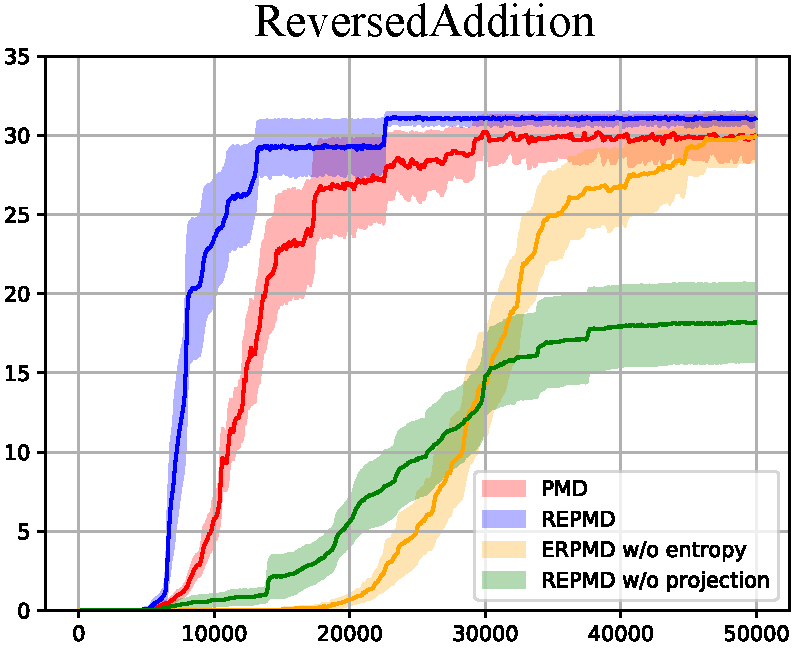
\includegraphics[width=0.35\linewidth]{ablation.pdf}}

\paragraph{Importance of entropy regularizer.} The main difference between the objective in \cref{eq:repmd} and the PMD
objective \cref{eq:pmd} is the entropy regularizer.
We demonstrate the importance of this choice by presenting the results of REPMD and PMAC without the extra entropy regularizer, i.e. $\tau'=0$.

\paragraph{Importance of KL divergence projection.} Another important difference between \cref{eq:repmd} with other RL methods
is to use a Project Step to update the policy,
rather than one SGD.
To show the importance of the Project Step,
we test REPMD and PMAC without projection,
which only performs one step of gradient update at each iteration of training. 

\paragraph{Importance of direction of KL divergence.} We choose PMD \cref{eq:pmd} as another baseline
to prove the effectiveness of using the \emph{mean seeking}
direction of KL divergence in the project step.
Similar to REPMD, we add a separate temperature parameter $\tau' > 0$
to the original objective function in \cref{eq:pmd}
to encourage policy exploration,
which gives
$\argmax_{\pi_\theta \in \Pi}{ \ep_{\rho \sim \pi_\theta}{  r(\rho)  - \tau \text{KL}(\pi_\theta \| \refPi) } + \tau'\cH(\pi_\theta) }$.
We name it PMD+entropy.
The corresponding algorithms in the actor-critic setting,
named PMD-AC and PMD-AC+entropy, are also implemented for comparison.

\begin{figure*}[t]
\begin{center}
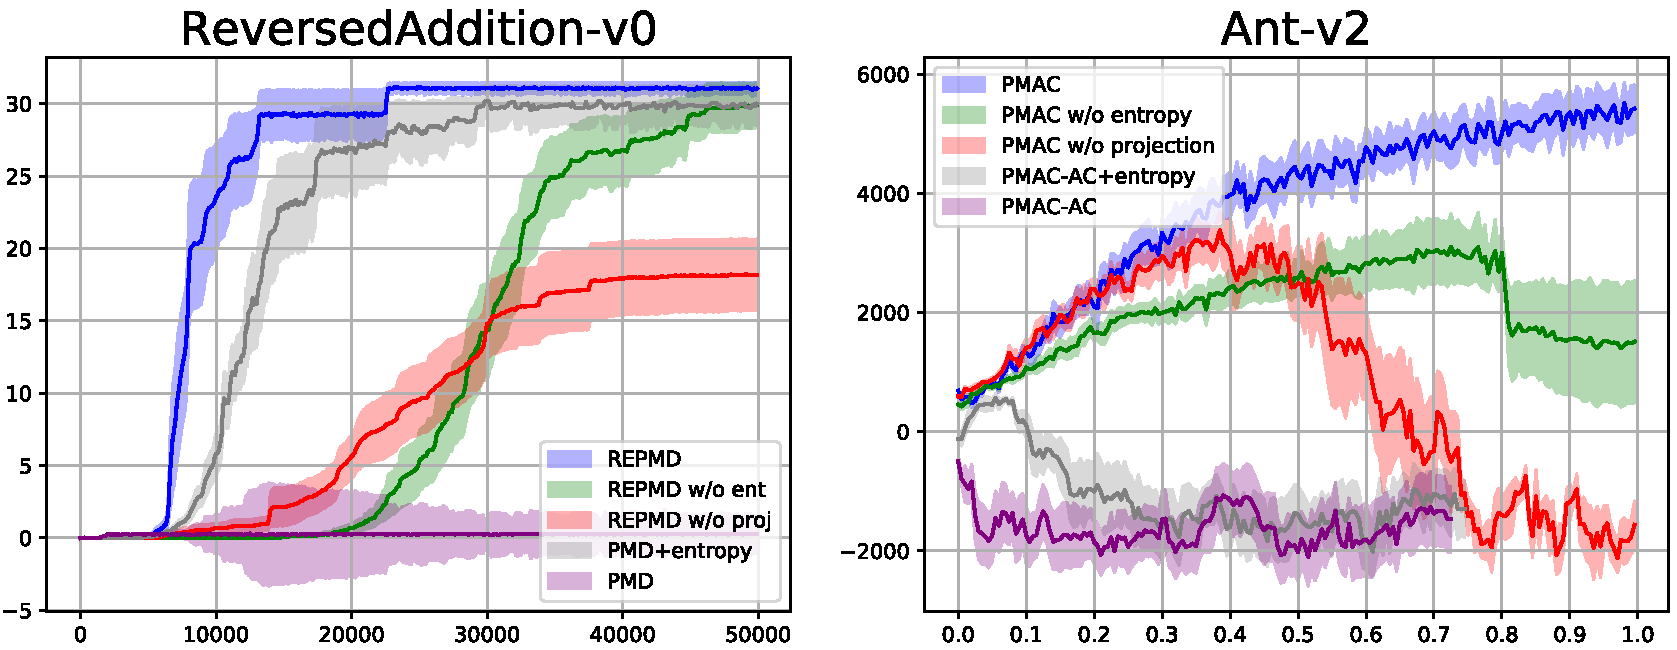
\includegraphics[width=0.5\linewidth]{./ablation-results.pdf}
\end{center}
\caption{Ablation Study of REPMD and PMAC %with designed baselines
on ReversedAddition and Ant. }
\label{fig:ablation}
\end{figure*}

The results are presented in \cref{fig:ablation},
which clearly indicate all of the three major components of \cref{eq:repmd}
are helpful for achieving better performance. 

